\chapter{Results}
\label{ch:results}

This chapter reports the experiments in the order they were carried out. Two
intermediate findings did not survive repetition: a hyperparameter configuration
that initially appeared promising (Section~\ref{sec:results-alpha0-validation})
and a two-run estimate that proved inconclusive
(Section~\ref{sec:results-mode-sweep}). Both are reported, since they motivated
the repeated-run protocol described in Chapter~\ref{ch:methodology},
Section~\ref{sec:methodology-rm-eval}, and omitting them would misrepresent how
much of the final estimate rests on distinguishing an effect from run-to-run
variance. Sections~\ref{sec:results-formula-opt} to~\ref{sec:results-mode-sweep}
are exploratory in the sense of Chapter~\ref{ch:methodology},
Section~\ref{sec:methodology-exploratory}; Section~\ref{sec:results-scale}
examines how the selected configuration behaves as the dataset grows.

\section{Early Prototype Results (Historical Context)}
\label{sec:results-early}

An earlier version of the pipeline produced results under a DPO-based design
before the study narrowed to reward-model comparison
(Chapter~\ref{ch:methodology}, Section~\ref{sec:methodology-evolution}). They are
reported here as context for that change, not as findings of the present study.

A FLAN-T5 baseline on a 20-sample pilot gave
ROUGE-1 0.3278, ROUGE-2 0.1201, ROUGE-L 0.2341, and BERTScore F1 0.8612. On a
200-sample subset (subset seed 42), the original AlignScore-based preference
construction, using the proposal-era margin of 0.05 and $\alpha = 0.5$, produced 154
usable holistic pairs out of 200 (77.0\%, mean scores 0.7324 for the low-temperature
candidate and 0.6530 for the high-temperature one) and 157 usable GCA pairs
(78.5\%, mean GCA scores 0.4066 and 0.3337). The two methods agreed on 121 of 200
decisions (60.5\%).

Mistral-7B-Instruct-v0.3 was then fine-tuned with DPO on both preference sets
(Chapter~\ref{ch:background}, Section~\ref{sec:bg-dpo}): training loss reached
0.6902 for the holistic condition and 0.6913 for the GCA condition, each in
roughly 134.5 seconds on an A100. On 200 held-out articles, baseline AlignScore was
0.7965, DPO-Holistic reached 0.8017, and DPO-GCA reached 0.7996. Only DPO-GCA's
ROUGE-L differed from baseline at the conventional threshold (Wilcoxon
$p=0.015$); the AlignScore differences between conditions were small and not
distinguishable from noise. These downstream results illustrate the attribution
problem described in Chapter~\ref{ch:methodology},
Section~\ref{sec:methodology-evolution}: differences of this magnitude cannot be
traced to the preference-construction procedure rather than to the optimization
stage, which is why the final study measures the preference data directly.

\section{Bradley--Terry Reward-Model Baseline}
\label{sec:results-rm-baseline}

The first Bradley--Terry reward-model result used the $n=495$ set (subset seed
100) with a \texttt{microsoft/deberta-v3-base} backbone, predating the
standardization on \texttt{FacebookAI/roberta-base}
(Chapter~\ref{ch:implementation}, Section~\ref{sec:impl-rm-training}). Under 5-fold
cross-validation, the holistic reward model reached 58.1\% mean pairwise accuracy
and the GCA reward model reached 54.6\%, both above the 50\% chance level.

The first result on the $n=1{,}000$ set, with the \texttt{roberta-base} backbone
and the original configuration ($\alpha = 0.5$, margin 0.05), is summarized in
Table~\ref{tab:rm-baseline-1000}. This is the baseline the rest of this chapter's
optimization campaign works from: holistic outperforms GCA by 1.2 percentage
points.

\begin{table}[htbp]
\centering
\caption[Bradley--Terry reward-model baseline at $n=1{,}000$]{Bradley--Terry reward-model baseline at $n=1{,}000$ ($\alpha=0.5$,
margin $0.05$, \texttt{roberta-base}).}
\label{tab:rm-baseline-1000}
\begin{tabular}{lrr}
\toprule
Condition & Mean pairwise accuracy & Gap (GCA $-$ Holistic) \\
\midrule
Holistic RM & 57.20\% & \multirow{2}{*}{$-1.20$ pp} \\
GCA RM      & 56.00\% & \\
\bottomrule
\end{tabular}
\end{table}

\section{GCA Formula Optimization}
\label{sec:results-formula-opt}

To understand why GCA underperformed, disagreement between the holistic and GCA
decisions at $\alpha = 0.5$ was analyzed directly on the $n=1{,}000$ pairs
(\texttt{analysis/gca\_vs\_holistic\_analysis.py}). The two methods disagreed on
17.8\% of pairs. GCA scores showed higher discrimination between candidates than
holistic scores (mean absolute score difference 0.2392 versus 0.1527), but only
82.2\% of GCA decisions agreed with the corresponding holistic decision, suggesting
that the extra discrimination was at least partly noise rather than signal.

Nine aggregation strategies were then compared by how well each agreed with the
holistic decision on the same 1{,}000 pairs
(\texttt{analysis/test\_gca\_formulas.py}, \texttt{analysis/test\_advanced\_aggregation.py}).
Table~\ref{tab:formula-comparison} reports the results. The simple mean
($\alpha = 0.0$) had the highest agreement of any strategy tested, 15.4 percentage
points above the original penalty formula.

\begin{table}[htbp]
\centering
\caption[Agreement with the holistic decision across nine aggregation strategies]{Agreement with the holistic decision across nine GCA aggregation
strategies, $n=1{,}000$ pairs.}
\label{tab:formula-comparison}
\begin{tabular}{lrr}
\toprule
Strategy & Agreement with holistic & vs.\ $\alpha=0.5$ baseline \\
\midrule
Simple mean ($\alpha=0.0$)   & 97.6\% & $+15.4$ pp \\
Confidence-weighted          & 96.0\% & $+14.0$ pp \\
Ensemble                     & 93.3\% & $+11.1$ pp \\
Length-weighted              & 91.5\% & $+9.3$ pp \\
Weighted by position         & 88.2\% & $+6.0$ pp \\
Robust mean (10\% trim)      & 85.4\% & $+3.2$ pp \\
Harmonic mean                & 82.9\% & $+0.7$ pp \\
Original penalty ($\alpha=0.5$) & 82.2\% & baseline \\
Minimum                      & 78.7\% & $-3.5$ pp \\
\bottomrule
\end{tabular}
\end{table}

\begin{figure}[htbp]
\centering
\begin{tikzpicture}
\begin{axis}[
  thesisplot,
  width=0.80\textwidth, height=6.2cm,
  xbar, bar width=8pt,
  xmin=70, xmax=100,
  xlabel={agreement with the holistic decision (\%)},
  ytick=data,
  symbolic y coords={Minimum,{Penalty $\alpha{=}0.5$},Harmonic mean,
                     Robust mean,Position-weighted,Length-weighted,
                     Ensemble,Confidence-weighted,{Simple mean $\alpha{=}0.0$}},
  y dir=reverse,
  nodes near coords, nodes near coords style={font=\scriptsize},
  every node near coord/.append style={/pgf/number format/fixed,
        /pgf/number format/fixed zerofill, /pgf/number format/precision=1},
]
\addplot[gcabar] coordinates {
  (78.7,Minimum) (82.2,{Penalty $\alpha{=}0.5$}) (82.9,Harmonic mean)
  (85.4,Robust mean) (88.2,Position-weighted) (91.5,Length-weighted)
  (93.3,Ensemble) (96.0,Confidence-weighted) (97.6,{Simple mean $\alpha{=}0.0$})};
\end{axis}
\end{tikzpicture}
\caption[Agreement across the nine aggregation strategies]{Agreement with the holistic decision across the nine aggregation
strategies of Table~\ref{tab:formula-comparison} ($n=1{,}000$ pairs). Agreement
measures consistency between two procedures driven by the same evaluator, not
external factual correctness.}
\label{fig:formula-agreement}
\end{figure}

On the strength of this result, the default $\alpha$ was changed from 0.5 to 0.0
throughout the codebase (\url{src/judging/gca.py},
\url{src/judging/build_reward_preferences.py}, and every Slurm script).

Two qualifications apply to this selection. First, the criterion used in
Table~\ref{tab:formula-comparison} is agreement with the holistic decision, which
is a measure of internal consistency between two procedures driven by the same
evaluator, not a measure of external factual correctness. A strategy could agree
closely with holistic scoring while reproducing the same errors, and nothing in
this comparison would distinguish those cases. The criterion is used here as a
diagnostic for whether the penalty term was amplifying disagreement, not as
evidence that the simple mean produces better labels. Second, this comparison and
the evaluator-mode sweep that follows are exploratory in the sense defined in
Chapter~\ref{ch:methodology}, Section~\ref{sec:methodology-exploratory}: the final
configuration was chosen after observing $n=1{,}000$ outcomes, so results on that
setting cannot also serve as independent confirmation of the choice. The
$n=5{,}000$ and $n=10{,}000$ experiments do not fully remedy this, because their
subsets are nested supersets of the $n=1{,}000$ set rather than independent
samples (Chapter~\ref{ch:methodology}, Section~\ref{sec:methodology-nesting}).

\section{Does the Formula Change Alone Flip the Result?}
\label{sec:results-alpha0-validation}

The formula change was then validated the same way the baseline was measured: by
training reward models on the resulting preferences and checking pairwise
accuracy, holding the judge mode fixed at the original \texttt{nli\_sp} setting.
Table~\ref{tab:alpha0-validation} shows that $\alpha = 0.0$ did not, on its own,
close the gap. Holistic accuracy improved more than GCA accuracy did, and the gap
between them widened slightly rather than closing.

\begin{table}[htbp]
\centering
\caption[Effect of the aggregation-formula change alone]{Effect of the formula change alone ($n=1{,}000$, judge mode
\texttt{nli\_sp} unchanged).}
\label{tab:alpha0-validation}
\begin{tabular}{lrrr}
\toprule
Metric & $\alpha=0.5$ (baseline) & $\alpha=0.0$ & Change \\
\midrule
Holistic mean accuracy & 0.572 & 0.586 & $+0.014$ \\
GCA mean accuracy      & 0.560 & 0.561 & $+0.001$ \\
Gap (Holistic $-$ GCA) & 0.012 & 0.025 & $+0.013$ (wider) \\
\bottomrule
\end{tabular}
\end{table}

A nine-configuration hyperparameter search was run next, sweeping learning rate
over $\{1\times10^{-5}, 2\times10^{-5}, 5\times10^{-5}\}$ and epoch count over
$\{3, 5, 7\}$, still at $\alpha = 0.0$. One configuration, learning rate
$1\times10^{-5}$ with 7 epochs, produced a GCA advantage of $+0.014$ (GCA 0.586
versus holistic 0.572). A same-seed confirmation rerun of that exact
configuration, however, produced the opposite result: holistic 0.577 versus GCA
0.560, a gap of $-0.017$. The apparent advantage did not reproduce. This result
is reported in full because of what it implies: at this dataset size, a single
training run, even with 5-fold cross-validation, can produce a result that looks
like a real effect but is actually within the range of ordinary fold-to-fold and
initialization noise. This directly motivated moving away from hyperparameter
tuning toward the judge-mode sweep below, and toward the multi-seed validation
protocol used for the headline result.

\section{AlignScore Judge-Mode Sweep}
\label{sec:results-mode-sweep}

With $\alpha = 0.0$ fixed, four AlignScore evaluation modes
(Chapter~\ref{ch:background}, Section~\ref{sec:bg-alignscore}) were compared under
the same $n=1{,}000$ training setup. Table~\ref{tab:mode-sweep} shows that the
choice of mode, not only the aggregation formula, is associated with whether GCA
leads at all. The \texttt{nli} mode produced the largest GCA
advantage of any configuration tested so far; \texttt{nli\_sp}, the mode used for
every result up to this point, is actually one of the two modes that favor
holistic.

\begin{table}[htbp]
\centering
\caption[AlignScore evaluator-mode sweep]{AlignScore judge-mode sweep ($n=1{,}000$, $\alpha=0.0$).}
\label{tab:mode-sweep}
\begin{tabular}{lrrr}
\toprule
Mode & Holistic mean acc.\ & GCA mean acc.\ & Gap (GCA $-$ Holistic) \\
\midrule
\texttt{nli}    & 0.523 & 0.583 & $+0.060$ \\
\texttt{bin}    & 0.510 & 0.564 & $+0.054$ \\
\texttt{bin\_sp} & 0.554 & 0.562 & $+0.008$ \\
\texttt{nli\_sp} & 0.578 & 0.557 & $-0.021$ \\
\bottomrule
\end{tabular}
\end{table}

Figure~\ref{fig:mode-sweep} plots the same values grouped by whether the
evaluator performs its own internal splitting.

\begin{figure}[htbp]
\centering
\begin{tikzpicture}
\begin{axis}[
  thesisplot,
  width=0.82\textwidth, height=5.6cm,
  ybar, bar width=13pt,
  ymin=0.48, ymax=0.62,
  ylabel={mean pairwise accuracy},
  symbolic x coords={nli,bin,bin\_sp,nli\_sp},
  xtick=data,
  legend style={at={(0.5,-0.22)}, anchor=north, legend columns=2},
  nodes near coords, nodes near coords style={font=\scriptsize,
        /pgf/number format/fixed, /pgf/number format/precision=3},
]
\addplot[holbar] coordinates {(nli,0.523) (bin,0.510) (bin\_sp,0.554) (nli\_sp,0.578)};
\addplot[gcabar] coordinates {(nli,0.583) (bin,0.564) (bin\_sp,0.562) (nli\_sp,0.557)};
\draw[dashed, gray!70] ({rel axis cs:0,0}|-{axis cs:nli,0.5}) --
                       ({rel axis cs:1,0}|-{axis cs:nli,0.5});
\node[font=\scriptsize, gray!60!black, anchor=south east]
      at ({rel axis cs:0.995,0}|-{axis cs:nli,0.5}) {chance};
\legend{Holistic, GCA}
\end{axis}
\end{tikzpicture}
\caption[Evaluator-mode sweep]{Evaluator-mode sweep ($n=1{,}000$, $\alpha=0.0$). The two left-hand
modes do not split the input internally; the two right-hand modes do. Each bar is
a single run, so differences of this size fall within the run-to-run variation
documented in Section~\ref{sec:results-final-campaign}, and the comparison is
exploratory.}
\label{fig:mode-sweep}
\end{figure}

The ordering in Table~\ref{tab:mode-sweep} follows a systematic pattern rather
than varying arbitrarily. The two modes in which GCA leads by a clear margin,
\texttt{nli} and
\texttt{bin}, are precisely the two that operate on the context and claim without
splitting them. The two modes in which the advantage is negligible or negative,
\texttt{bin\_sp} and \texttt{nli\_sp}, are the split variants, in which the
evaluator itself segments the input and aggregates over the segments
(Chapter~\ref{ch:background}, Section~\ref{sec:bg-alignscore}). Holistic accuracy
also rises from 0.510--0.523 in the unsplit modes to 0.554--0.578 in the split
modes, which is consistent with the split modes supplying a stronger holistic
signal rather than with GCA becoming worse.

The pattern suggests that external sentence-level decomposition may contribute
most where the evaluator does not already decompose internally, and little where
it does; on this reading GCA and the evaluator's own splitting act partly as
substitutes. This sweep is exploratory and each mode was run once, so the
comparison across modes should be read as suggestive rather than established:
Section~\ref{sec:results-final-campaign} shows that single-run differences of this
magnitude fall within the range of run-to-run variation, and only the
\texttt{nli} configuration was subsequently validated across repeated runs.
Chapter~\ref{ch:discussion}, Section~\ref{sec:disc-interpretation} develops the
interpretation and states what would be required to test it.

Because a single run had already proved insufficient in
Section~\ref{sec:results-alpha0-validation}, the \texttt{nli} result was rerun at
the same seed value before any conclusion was drawn. The rerun gave holistic 0.543
and GCA 0.556, a gap of $+0.013$: smaller than the original $+0.060$, but in the
same direction. Over the fold-level differences from both runs, the 95\% interval
was $[+0.003, +0.064]$ and the corresponding Wilcoxon $p$-value was 0.084. Under
the independence caveat discussed above, neither figure was treated as decisive,
and further runs were carried out rather than concluding from two.

\section{Repeated Runs of the Selected Configuration (\texorpdfstring{$n=1{,}000$}{n=1,000})}
\label{sec:results-final-campaign}

The \texttt{nli} mode, $\alpha=0.0$, margin 0 configuration was fixed and run
across four further seed values, in addition to the original sweep and its
confirmation rerun, for six runs and 30 cross-validation folds in total.
Table~\ref{tab:seed-validation} lists every run. Note that the six runs span five
distinct seed values, not six: seed 42 appears twice, as the original sweep and
its rerun. As discussed in Chapter~\ref{ch:methodology},
Section~\ref{sec:methodology-rm-eval}, those two runs are not duplicates, because
the seed argument controls only fold assignment and not the reward model's weight
initialization.

\begin{table}[htbp]
\centering
\caption[Per-run results for the selected configuration]{Per-run results for the selected \texttt{nli}-mode configuration
($n=1{,}000$).}
\label{tab:seed-validation}
\begin{tabular}{lrrrr}
\toprule
Run & Seed & Holistic & GCA & Gap (GCA $-$ Holistic) \\
\midrule
Original sweep       & 42   & 0.523 & 0.583 & $+0.060$ \\
Confirmation          & 42   & 0.543 & 0.556 & $+0.013$ \\
Seed validation 1    & 7    & 0.556 & 0.546 & $-0.010$ \\
Seed validation 2    & 100  & 0.510 & 0.561 & $+0.051$ \\
Seed validation 3    & 314  & 0.520 & 0.552 & $+0.032$ \\
Seed validation 4    & 2026 & 0.525 & 0.564 & $+0.039$ \\
\bottomrule
\end{tabular}
\end{table}

GCA leads in five of the six runs; seed 7 is the only run in which holistic is
ahead. Figure~\ref{fig:per-run-gaps} plots the per-run gaps against the pooled
mean, which makes the spread easier to judge than the table alone: the individual
runs range from $-0.010$ to $+0.060$, a spread wide enough that any single run,
taken on its own, would have been weak evidence in either direction. Averaging
over all 30 fold-level readings gives the central estimate of this thesis, shown
in Table~\ref{tab:pooled-headline}: a mean gap of $+3.08$ percentage points.

\begin{figure}[htbp]
\centering
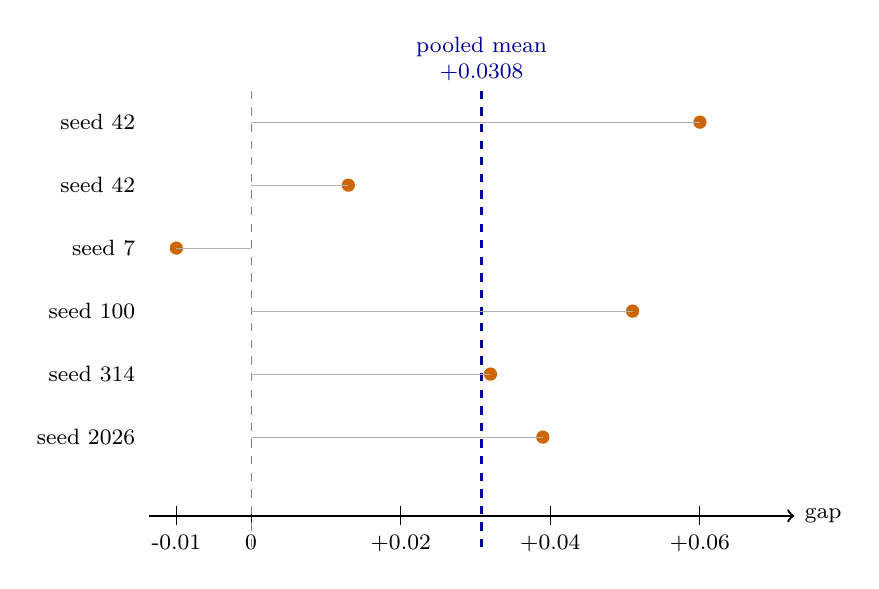
\begin{tikzpicture}[font=\footnotesize]
  % axes
  \def\xz{0}      % x origin
  \def\xs{95}     % x scale (per 0.01 gap) -- gaps range -0.01..0.06
  \draw[->, thick] (-1.3,0) -- (6.9,0) node[right] {gap};
  \foreach \g/\lab in {-0.01/-0.01, 0/0, 0.02/+0.02, 0.04/+0.04, 0.06/+0.06} {
    \draw ({\g*\xs},0.12) -- ({\g*\xs},-0.12) node[below] {\lab};
  }
  % zero reference line
  \draw[dashed, gray] (0,-0.4) -- (0,5.4);
  % pooled mean line
  \draw[thick, blue!60!black, dashed] ({0.0308*\xs},-0.4) -- ({0.0308*\xs},5.4);
  \node[blue!60!black, anchor=south, align=center] at ({0.0308*\xs},5.4)
    {pooled mean\\$+0.0308$};
  % runs (y from top to bottom)
  \foreach \y/\seed/\gap in {
      5/42/0.060,
      4.2/42/0.013,
      3.4/7/-0.010,
      2.6/100/0.051,
      1.8/314/0.032,
      1.0/2026/0.039} {
    \node[anchor=east] at (-1.35,\y) {seed \seed};
    \fill[orange!80!black] ({\gap*\xs},\y) circle (2.4pt);
    \draw[gray!60] (0,\y) -- ({\gap*\xs},\y);
  }
\end{tikzpicture}
\caption[Per-run GCA$-$Holistic accuracy gap at $n=1{,}000$]{Per-run GCA$-$Holistic accuracy gap at $n=1{,}000$, against the pooled
mean. Five of six runs favor GCA, but the spread across runs is wide relative to
the pooled effect, which is why no single run was treated as conclusive.}
\label{fig:per-run-gaps}
\end{figure}

\begin{table}[htbp]
\centering
\caption[Averaged result across six runs at $n=1{,}000$]{Averaged result across 6 runs / 30 cross-validation folds at
$n=1{,}000$. The interval and $p$-value are computed over folds, which are not
independent observations, and are therefore exploratory and anti-conservative
(Chapter~\ref{ch:methodology}, Section~\ref{sec:methodology-rm-eval}).}
\label{tab:pooled-headline}
\begin{tabular}{rrrrr}
\toprule
Holistic mean & GCA mean & Gap & 95\% fold-level CI & Fold-level Wilcoxon $p$ \\
\midrule
0.5295 & 0.5603 & \textbf{+0.0308} & $[+0.013, +0.047]$ & 0.0034 \\
\bottomrule
\end{tabular}
\end{table}

At the fold level, GCA leads in 22 of the 30 folds (73\%), with no ties. The
interval and $p$-value in Table~\ref{tab:pooled-headline} are computed as
described in Chapter~\ref{ch:background}, Section~\ref{sec:bg-stats}, using
10{,}000 bootstrap resamples with a fixed NumPy seed of 42.

These uncertainty estimates require an explicit caveat and are not presented as
confirmatory. The 30 folds are not 30 independent observations: the five folds
within a run partition one dataset, so their training sets overlap heavily and
their errors are correlated. A procedure that assumes independence therefore
treats the evidence as stronger than it is, and the quoted $p$-value is
anti-conservative. What the fold-level analysis supports is that the difference is
consistent in direction across runs and stable in magnitude, not that it meets a
particular significance threshold. Chapter~\ref{ch:discussion},
Section~\ref{sec:disc-stats-caveat} examines what a more conservative treatment
would and would not permit.

A second property should be read alongside the gap. Both conditions sit close to
chance in absolute terms: 0.5295 and 0.5603 are 2.95 and 6.03 percentage points
above the 0.5 chance level. The comparison is therefore between two weak
preference signals, and the finding concerns which is more consistently
recoverable, not whether either yields a strong reward model
(Section~\ref{sec:disc-weak-signal}).

Table~\ref{tab:evidence-progression} tracks how the estimate changed as runs were
added. The interval narrows at each stage while the point estimate stays near
three percentage points. Stability of the effect size as precision improves is
consistent with a real underlying difference rather than with an artifact that
grows as data accumulates, though the same independence caveat applies to every
row of the table.

\begin{table}[htbp]
\centering
\caption[Progression of the pooled estimate as runs were added]{Progression of the pooled statistical estimate as runs were added. The
$p$-values are subject to the independence caveat discussed in
Chapter~\ref{ch:discussion}, Section~\ref{sec:disc-stats-caveat}.}
\label{tab:evidence-progression}
\begin{tabular}{lrrrrr}
\toprule
Stage & Runs & Folds & Pooled gap & 95\% CI & Wilcoxon $p$ \\
\midrule
Two-run  & 2 & 10 & $+0.034$ & $[+0.003, +0.064]$ & 0.084 \\
Five-run & 5 & 25 & $+0.029$ & $[+0.009, +0.048]$ & 0.0123 \\
Six-run  & 6 & 30 & $+0.031$ & $[+0.013, +0.047]$ & 0.0034 \\
\bottomrule
\end{tabular}
\end{table}

\section{Scale Robustness: 5{,}000 and 10{,}000 Samples}
\label{sec:results-scale}

The selected configuration was then run once at $n=5{,}000$ and once at
$n=10{,}000$. These subsets are nested supersets of the $n=1{,}000$ set rather
than independent samples (Chapter~\ref{ch:methodology},
Section~\ref{sec:methodology-nesting}), so they measure how the effect behaves as
data is added to the same pool rather than providing out-of-sample replication.
Unlike the
$n=1{,}000$ result, each of these runs is a single run, not a six-run pool, for
computational-budget reasons stated in Chapter~\ref{ch:methodology},
Section~\ref{sec:methodology-rm-eval}; the comparison in
Table~\ref{tab:scale-robustness} should be read with that difference in mind
rather than treated as three results of equal statistical weight.

\begin{table}[htbp]
\centering
\caption[Selected configuration at three dataset sizes]{Selected configuration at three dataset sizes. Only the $n=1{,}000$ row
is averaged over repeated runs; the other two are single runs on nested datasets.}
\label{tab:scale-robustness}
\begin{tabular}{rrrr}
\toprule
Dataset size & Holistic mean & GCA mean & Gap (GCA $-$ Holistic) \\
\midrule
1{,}000  & 0.5295 & 0.5603 & $+0.0308$ \\
5{,}000  & 0.5788 & 0.5746 & $-0.0042$ \\
10{,}000 & 0.5827 & 0.5862 & $+0.0035$ \\
\bottomrule
\end{tabular}
\end{table}

\begin{figure}[htbp]
\centering
\begin{tikzpicture}
\begin{axis}[
  thesisplot,
  width=0.82\textwidth, height=5.6cm,
  ybar, bar width=15pt,
  ymin=0.48, ymax=0.63,
  ylabel={mean pairwise accuracy},
  xlabel={preference pairs},
  symbolic x coords={1{,}000,5{,}000,10{,}000},
  xtick=data,
  legend style={at={(0.03,0.97)}, anchor=north west, legend columns=1},
]
\addplot[holbar] coordinates {(1{,}000,0.5295) (5{,}000,0.5788) (10{,}000,0.5827)};
\addplot[gcabar] coordinates {(1{,}000,0.5603) (5{,}000,0.5746) (10{,}000,0.5862)};
\draw[dashed, gray!70] ({rel axis cs:0,0}|-{axis cs:1{,}000,0.5}) --
                       ({rel axis cs:1,0}|-{axis cs:1{,}000,0.5});
\node[font=\scriptsize, gray!60!black, anchor=south west]
      at ({rel axis cs:0.30,0}|-{axis cs:1{,}000,0.5}) {chance};
\legend{Holistic, GCA}
\end{axis}
\end{tikzpicture}
\caption[Accuracy at the three dataset sizes]{Accuracy at the three dataset sizes. Absolute accuracy rises for both
conditions as data is added, while the difference between them contracts. Only
the $n=1{,}000$ bars are averaged over repeated runs; the other two are single
runs on datasets that are nested supersets of the $n=1{,}000$ set
(Chapter~\ref{ch:methodology}, Section~\ref{sec:methodology-nesting}).}
\label{fig:scale-results}
\end{figure}

The $n=1{,}000$ advantage is not reproduced with comparable magnitude at
$n=5{,}000$: holistic performs marginally better there, though the gap is small.
At $n=10{,}000$ the direction returns in GCA's favor, but the magnitude is an
order of magnitude smaller than at $n=1{,}000$. Neither larger-scale result was
repeated across runs the way the $n=1{,}000$ result was, so it cannot be ruled
out that some of this movement reflects the same run-to-run variation documented
in Section~\ref{sec:results-alpha0-validation} rather than a change in the
underlying effect as dataset size grows. What can be said without qualification is
that a single dataset size is not sufficient to characterize the difference
between the two conditions, and that reporting only $n=1{,}000$ would have
overstated how consistently the GCA advantage is observed.

\section{Summary of Results}
\label{sec:results-summary}

Table~\ref{tab:rq-summary} summarizes how the results in this chapter bear on the
research questions from Chapter~\ref{ch:methodology}, Section~\ref{sec:methodology-rqs}.
Full interpretation is left to Chapter~\ref{ch:discussion}.

\begin{table}[htbp]
\centering
\caption[Summary of findings against the research questions]{Summary of findings against the research questions.}
\label{tab:rq-summary}
\renewcommand{\arraystretch}{1.25}
\begin{tabularx}{\textwidth}{@{}>{\bfseries}l X@{}}
\toprule
& Finding \\
\midrule
RQ1 &
  At $n=1{,}000$, GCA leads in 5 of 6 runs with a mean difference of
  $+3.08$ percentage points. The run-level two-sided test does not meet
  $p<0.05$, and the larger single-run experiments do not reproduce an advantage
  of comparable magnitude. \\
RQ2 &
  Aggregation strategy and evaluator mode are associated with substantial
  outcome differences. The evaluator-mode comparison is exploratory, because
  every mode except the subsequently selected \texttt{nli} configuration was
  evaluated only once. \\
RQ3 &
  The direction is relatively stable across the six $n=1{,}000$ runs, but is not
  reproduced at comparable magnitude in the single $n=5{,}000$ and $n=10{,}000$
  runs, which use nested datasets. \\
\bottomrule
\end{tabularx}
\end{table}
